\section{Introduction}

In this chapter, I demonstrate that by modelling literature citations as
observations of a generative model with latent variables, research topics as
well as evolution themes of research can be identified and described inactively.
It also exemplifies that PLVM is an effective means to discover knowledge in
data mining problems.

How to leverage information technologies to improve the  productivity of
scientific research is a highly important challenge with clearly huge impact on
the society. One bottleneck in research productivity is that as a research
community grows, it would be increasingly difficult for researchers to see the
complete picture of how a field has been evolving, given the fact that large
volume new literatures are written based on previous works. Junior researchers
can often get lost in the overwhelming amount of related papers. Researchers who
seek to shift to a new topic may spend lots of time preparing a reading list on
his/her own. All these clearly hinder the progress of scientific research, and
it would be highly beneficial to develop mining techniques to help researchers
more easily and more efficiently  understand research themes in scientific
literature.  In general, two aspects of analysis are needed for understanding
research themes: First, we need to analyze \emph{each research topic} to answer
the following questions: Which papers are the milestone papers that best
represent a topic and how to quantify their impact?  When did the topic become
popular and is it still attracting attention today?  Can the topic be summarized
accurately with a few keywords?  Furthermore, when \emph{investigating topics
collectively}, which are the most dominant topics extensively studied?  During
the evolution, what are the newly generated topics initiated by the old one?
Can we identify the underlying evolution patterns among topics?

\begin{figure}[h!]
  \begin{center}
    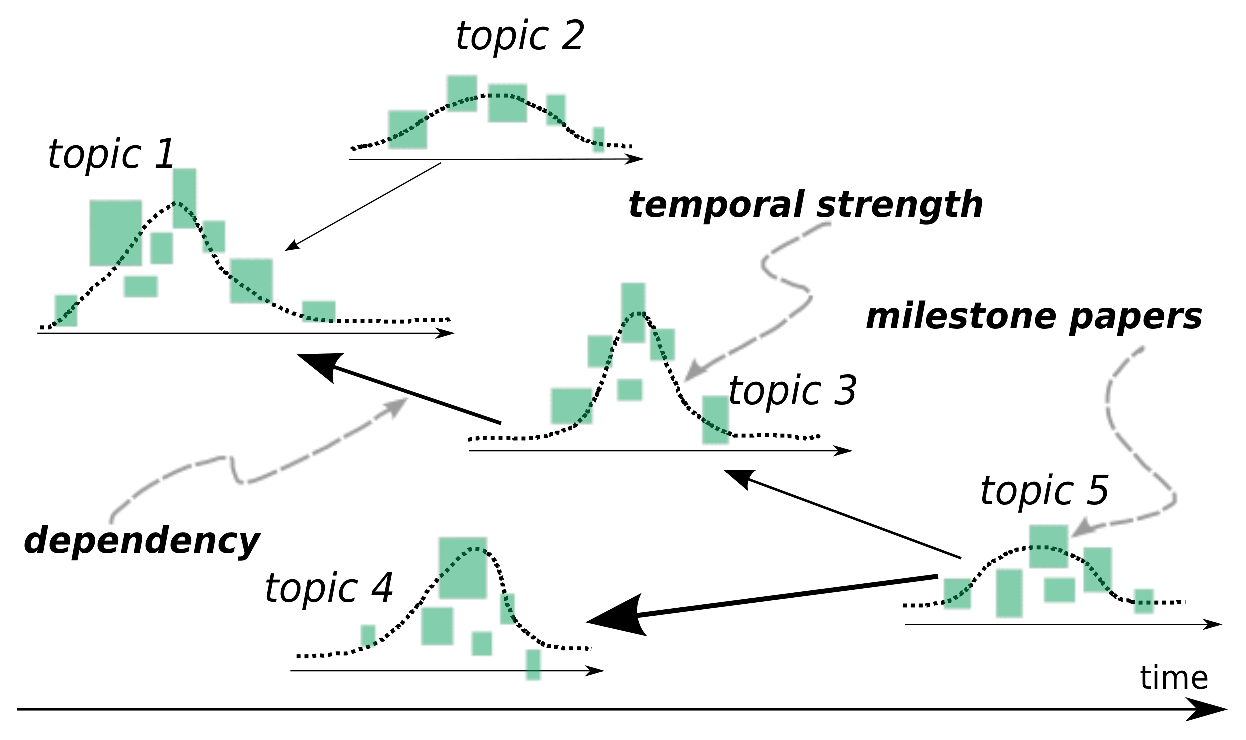
\includegraphics[scale= .6]{citation-lda/plot/fake_theme.eps}
  \end{center}
  \caption{An illustration of the proposed evolution graph. We show 5 topics,
  and their dependency. Topic 2 and 3 are enabled by Topic 1 while Topic 5 is
  enabled by Topic 3 and 4.}
  \label{fig::fake}
\end{figure}

To answer the questions raised above, ideally, we would like to automatically
construct a \emph{``research theme evolution graph''}, which we illustrate in
\Cref{fig::fake}.  With such a graph, when zooming into the scope of individual
topics, multiple types of information are provided to facilitate users to
understand the research topic:

\begin{itemize}
\item \emph{Topic Milestone Papers}: It is critical to recognize the papers that
  are best representative for a topic in the course of understanding topics. We
  refer to them as ``topic milestone papers''. Milestone papers of a topic
  provide a good picture how a topic is formed. In \Cref{fig::fake}, milestone
  papers are shown in each topic as rectangles and the ``size'' reflects their
  importance with respect to topics.
\item \emph{Topic Temporal Strength}: The relative popularity of topics at
  different times reveals the temporal nature of topics, which can help users to
  identify \emph{current} vs. \emph{previous} research topics as well as the
  rough topic life spans. Intuitively, when many milestone papers occur, the
  topic draws more attention and becomes popular.
\item \emph{Topic Keywords}: Extracting keywords that can properly summarize a
  topic would enable users to obtain a brief idea about the topic even without
  reading its relevant papers, allowing users to fast navigate among topics in
  search of the most interesting ones.
\end{itemize}

While zooming out to see the big picture of all related topics in the theme,
there is also meaningful information to explore:
\begin{itemize}
\item  \emph{Topic Importance}: Quantifying the importance of topics helps a
  user to discriminate the \emph{major} vs. \emph{minor} topics in a research
  theme. Topic importance also reflects how well the topic is recognized by the
  community.
\item \emph{Topic Dependency}: Many new topics are built on top of the old ones.
  Discovering the dependency relation between topics provides a good guidance
  for users when searching for \emph{origin/continuing} topics. In
  \Cref{fig::fake}, we visualize the dependency strength between topics by the
  ``thickness'' of edges.
\item \emph{Evolution Patterns}: Connecting topics by their dependency
  illustrates the underlying evolution patterns for research themes. Is there
  any trend that different topics get merged together to form a new
  (interdisciplinary) topic, such as Topic~3 and Topic~4 are merged into
  Topic~5? Or is there a general topic branched into multiple topics that
  address specialized problems, such as Topic~1 has led to Topic~2 and Topic~3?
\end{itemize}

To automatically construct such an evolution graph as shown in \Cref{fig::fake},
the two major computational tasks are:
\begin{itemize}
\item \textbf{\emph{Discovering the research topics}}, which includes finding
  milestone papers, computing the temporal strength, and extracting keywords for
  each individual topic.
\item \textbf{\emph{Discovering the theme evolution}}, which includes
  identifying the topic importance and learning the dependency relation between
  topics, as well as recognizing the underlying evolution patterns.
\end{itemize}

Existing approaches, notably those of topic modeling, can generate some (not
all) of these components in the evolution graph, but they are far from adequate
for the following reasons: First, though there are many works that aim to
construct evolution map over time, they rely on pre-segmentation of text streams
into fixed time windows, due to either computational
issue~\cite{blei2006dynamic,mei2005discovering,wang2006topics} or modeling
issue~\cite{wang2012continuous}. Consequently, the topic evolution result would
be inevitably sensitive to the choice of temporal granularity of how time is
discretized and sliced. Suboptimal granularity of time might result in missing
important topics or even lead to inaccurate evolution analysis.  Second, the
edges in most of the existing evolution graphs, do not reflect the
\emph{dependency relation} between topics, and can only reveal the \emph{topic
similarity} and \emph{correlation}
~\cite{blei2006dynamic,blei2007correlated,mei2005discovering,wang2012continuous}.
The fundamental limitation is that content-based topic modeling approaches are
built on \emph{word co-occurrence}, which essentially is \emph{undirected}
unlike the dependency relation.  Third, it is difficult for any aforementioned
models (including Pairwise Link-LDA~\cite{nallapati2008joint}) to assess the
impact of documents with respect to different topics, i.e., identifying the
milestone papers. Their approaches model topics as distributions over words, and
although the text similarity between document and topic can be computed, it
would be a substantially different measurement from the document \emph{impact}
on a topic.

As hinted above, a major reason why existing topic models are insufficient is
that they have not fully exploited citation relations to discover topics. In
this chapter, we address these limitations by doing joint analysis of citations
and text.  Indeed, we will rely  more on citation links than on document
content, which makes our work different from~\cite{nallapati2008joint} and all
others. Specifically, we leverage a similar idea to topic modeling and analyze
the citation graphs in a \emph{probabilistic} manner. We directly model the
generation of citations, which are direct evidence related to \emph{``impact''}
of document as well as \emph{``dependency''} between topics. Through citation
generation, we are enabled to address the core problem of assessing milestone
papers based on impact, and estimating the topic dependency.  More importantly,
our key insight here is that ``co-cited papers'' are good indicators of research
topics, more effective than relying on text similarity as in most existing work.
Empirical study~\cite{boyd2009reading} has already noticed that it is a
subjective yet difficult task to annotate for each word its belonging topic even
manually. However, for citations in a published paper written by experienced
authors, it would be much easier to determine the topic since most authors make
citations prudently and thus citation is much \emph{less noisy} than text.

To discover topics based on citations, we propose a novel probabilistic approach
to analyze citations by viewing citation graphs as a set of ``citation
documents'' where each is a research paper represented as a \emph{``bag of
citations''}. A paper that cites $k$ other (possibly duplicated) papers would
simply be viewed as a \emph{``document''} with $k$ \emph{``tokens''}, each
corresponding to the ID of a cited paper. With this view, we can model all these
citation documents with a generative topic model where we introduce latent topic
variables over the citations. This is analogous to the application of a
probabilistic topic model to model topics in text documents, but with the
important difference that the discovered topics with our model would be
characterized by a (multinomial) \emph{distribution over research papers},
rather than over words as in conventional content-based topic models. In
addition, when combined together with additional information, particularly the
\emph{published time} and the \emph{title} of each paper, our model can address
the computational tasks of discovering both \emph{the research topics} and
\emph{the theme evolution}, and constructing \emph{the evolution graph} as well.

In the rest of the chapter, we first review some of the related work in
\Cref{sec::citation-related}, which is followed by presenting our probabilistic
model for literature citations in \Cref{sec::citation-model}. After the
derivation about one specific model Citation-LDA, we focus our discussion on how
to construct the theme evolution graph in \Cref{sec::citation-graph}. Experiment
setup and extensive evaluation results will be given in
\Cref{sec::citation-exp}. Finally, we conclude our work with future direction in
\Cref{sec::citation-conclusion}.

\section{Related Work}\label{sec::citation-related}

In recent years, many literature search engines as well as digital libraries
have come into use, including Microsoft Academic
Search~\footnote{http://academic.research.microsoft.com/}, Google
Scholar~\footnote{ http://scholar.google.com/}, DBLP~\footnote{
http://www.informatik.uni-trier.de/~ley/db/} and ACM Digital
Library~\footnote{http://dl.acm.org/}. They provide knowledge about scientific
literatures through ranking and search interface, which in turn, relies on
algorithms that utilize citation-related indicators such as
H-index~\cite{hirsch2005index} and Impact Factor~\cite{garfield2006history}.

In the research community, one thread of study treats scientific literature as
citation graphs. To assess the importance of papers, graph ranking algorithms
such as PageRank and its variants have been
applied~\cite{ghosh2011time,radev2009acl,sayyadi2009futurerank,walker2007ranking}.
In~\cite{ghosh2011time}, the authors further take time into consideration in
order to overcome the recency bias that favors ``old'' papers. Apart from this,
graph clustering is investigated to identify meaningful topics, such
as~\cite{bolelli2006clustering,flake2004graph,popescul2000clustering,
qazvinian2008scientific}. In~\cite{popescul2000clustering}, it is pointed out
that efficient graph clustering can be combined with temporal information to
identify the trends of topics in literature.  Particularly, one recent
paper~\cite{jo2011web} is close to our work. It leverages both citation and
text~(title and abstract) to generate the evolution map in computer science
community. Specifically, their method relies on the temporal order of papers and
the document language model to detect the formation of new topics, and then it
computes the strength between two topics with the ``cross citation
count''~(total citation numbers between the two topics), which however ignores
the directed relation of topic dependency.  Their method is difficult to be
applied to address our problem because their method does not distinguish the
difference in topic importance, nor does it recognize milestone papers through
assessing the impact based on citations.

While on the other hand, existing probabilistic topic modeling over
text~\cite{blei2003latent,griffiths2004finding,hofmann2001unsupervised} has been
throughly studied, treating documents as mixtures of latent topics.  Early
attempt in modeling the topic evolution~\cite{mei2005discovering} investigates
the Probabilistic Latent Semantic Index~(PLSI)~\cite{hofmann2001unsupervised} to
extract topics and models the evolution process as transitions between topics in
Hidden Markov Model~(HMM).  Later, Topic Over Time~(TOT)
model~\cite{wang2006topics} is developed based on Latent Dirichlet
Allocation~(LDA)~\cite{blei2003latent}. The key difference between between LDA
and TOT is that TOT explicitly assumes time as generated from topics, which
jointly models time and word, thus enabling itself to discover time-aware topics
as well as topic temporal strength.  Besides, Dynamic Topic
Models~\cite{blei2006dynamic,wang2012continuous} address the problem of topic
evolution by modeling topics~(distributions over words) changing over time. In
the discrete case~\cite{blei2006dynamic}, topics at the next time-stamp deviate
from the current ones by a Gaussian noise; while, in the continuous
case~\cite{wang2012continuous}, the change of topics over time is generalized as
Brownian motion.  One limitation of these models~\cite{blei2006dynamic,
mei2005discovering,wang2012continuous,wang2006topics} is that they all rely on
the pre-segmentation of time: without appropriate time granularity selected,
they could fall into difficulty in finding important topics. Ideally, the
selection of correct time span should be made automatically.  In addition to
these studies, others consider the problem of modeling topic
correlation~\cite{blei2007correlated} and document hyperlink
generation~\cite{chang2009relational}, for which the essential difficulty is
that they cannot model the \emph{``dependency''} relation between topics. The
only exception we are aware of so far is the paper~\cite{nallapati2008joint}
which jointly models text and citation generatively. One of its proposed model,
named ``Pairwise Link-LDA'', explicitly includes the topic dependency as model
parameters by extending the idea of mixed-membership block stochastic
models~\cite{airoldi2006mixed}. In words, the chance of generating a particular
citation is determined by the topics of citing and cited documents, which indeed
addresses the topic dependency directly. Nevertheless, the Pairwise Link-LDA is
not able to fulfill all the tasks we listed such as recognizing the milestone
papers and so on.


To our best knowledge, there is no existing approach that can address all the
questions as we raised before, i.e., the discovery of \emph{research topics} and
\emph{theme evolution}. To this end, we directly model the generation of the
citation links among literatures in this work. In the same spirit of topic
modeling, citations are generated stochastically according to a distribution
with respect to the underlying topic. It is worth noting that applying the topic
modeling approaches to study graphs was previously investigated for discovering
communities from coauthorship networks in
\cite{henderson2009applying,zhang2007lda}. Nevertheless, our model not only
discovers the topics, but also explores their dependency relationships and
yields meaningful knowledge about the evolution of topics.

\section{Probabilistic Modeling of Literature
Citations}\label{sec::citation-model}

In contrast to most existing work on citation analysis, where citations are
often modeled as network or graph, we propose to represent citation graph as a
set of ``citation documents'' where each is a research paper represented as
``bag of citations'', and model these citation documents with a probabilistic
generative model.  Such a new approach has several advantages over pure graph
analysis methods.  First, by using a latent topic variable, we can naturally
associate topics with papers and citations, enabling ranking the paper based on
citation within each topic, through which milestone papers can be identified.
Second, by modeling the whole set of papers in a field, we can obtain a set of
topics that summarize well the major research topics in the field, with
(probabilistic) weights quantifying their importance.  Third, by estimating the
topic level citation structure, it is possible to compute the strength of
dependency relation between topics and picturing the evolution paths of research
themes.  Last, distribution over papers for each topic obtained by such a model
can be easily used to compute a distribution over time or keywords when used
together with other information such as paper published time and title, allowing
modeling the topic temporal strength and summarizing topics with keywords.

Compared with pure content-based topic models, our use of topic model is
entirely on capturing topics through citation structures, roughly corresponding
to discovering topics based on \emph{co-citation relation}, which is intuitively
more accurate in finding research topics: if there is a \emph{``stable''} set of
\emph{``core papers''} that are often cited together, then it generally
indicates the existence of a major research topic and the core papers are
actually \emph{milestone papers} in that topic. Specifically, we use a
probabilistic model to explain how an author generates the references
(citations) for a paper (which we may also refer to as a document for
convenience sometimes).  More specifically, given a paper, he/she would
``generate'' all the references cited in the paper independently.  When
generating each citation, the author would first sample a topic according to a
document-specific topic distribution~($doc\_topic$ distribution), and then draw
a reference document to cite from the citation distribution of the sampled
topic~($topic\_doc$ distribution).  One may easily notice that such a generation
process is essentially similar to the one over words for documents assumed in
probabilistic topic models for text data.  Indeed, our work is a novel way of
using topic models for citation analysis, and just as topic models are very
effective for discovering and analyzing topics in \emph{text documents}, our
model can also be very useful for discovering and analyzing topics in
\emph{scientific literatures} where the citation graph is available. Another
advantage over content-based topic models we may anticipate is that the
computational complexity is greatly reduced because the number of citations is
much less than the number of words in the corpora.

\subsection{The General Model}

Formally, suppose each document $d$ cites a subset of other documents
$\{c_t\}$~$(t=1,2,\ldots)$, where $c_t$ is a cited reference. We
assume the following generation process for a citation that links to document
$c_t$ in document $d$ (i.e., document $d$ cites document $c_t$):

\begin{itemize}
\item  Draw topic sample: $z_t \sim D_{doc\_topic}(z;d)$
\item  Draw citation sample: $c_t \sim D_{topic\_doc}(c;z_t)$
\end{itemize}

The doc-topic distribution $D_{doc\_topic}(\cdot;d)$ and topic-doc distribution
$D_{topic\_doc}(\cdot;z)$ are parameterized by the citing document $d$ and the
topic $z$ respectively, and are the two key components in the model that would
enable many interesting ways to analyze topics and evolution relations among
topics.  Indeed, $D_{doc\_topic}(\cdot;d)$ gives us a probability distribution
over (latent) topics conditioned on document $d$, and can be interpreted as the
\emph{topic coverage} in document $d$ when generating citations, whereas
$D_{topic\_doc}(\cdot;z)$ gives a \emph{``reverse''} conditional distribution of
documents given a topic, and can be interpreted as how a topic is characterized
by a set of papers (documents) that are cited.  Thus if a document $c_i$ has a
higher probability than $c_j$  according to  $D_{topic\_doc}(\cdot;z)$, it would
suggests that $c_i$ better characterizes topic $z$ than $c_j$, or $c_i$
represents topic $z$ better as being a more important paper with higher impact
upon $z$ than $c_j$.  With such a distribution over papers, we can easily
compute the \emph{expected time} for a topic based on the time when the paper
was published as well as the \emph{topic keywords} based on the paper titles (or
abstracts if available).  Note that a substantial advantage of such a
probabilistic model is that it can \emph{``decode''} why document $d$ cites
document $c_t$ by inferring the latent topic associated with this citation
relation and quantifying with uncertainty, which enables ``disambiguation'' of
citation relations to some extent.  As will be further discussed, we can use
such a model to perform the computational analysis for discovering research
topics and theme evolution, which finally lead to the construction of evolution
graph as proposed in \Cref{fig::fake}.


\subsection{Citation-LDA}

Though we may have different ways to refine the general probabilistic model
defined above, in this work as a first step, we focus on exploring the use of
the basic Latent Dirichlet Allocation (LDA)~\cite{blei2003latent} model, which
we call ``Citation-LDA'' and show that even with this simple model setting, we
can already discover a lot of interesting knowledge that is useful for
understanding research theme evolution.

Specifically, Citation-LDA assumes that $D_{doc\_topic}$ and $D_{topic\_doc}$
are multinomial distributions with parameters drawn from conjugated Dirichlet
prior $\alpha$ and $\beta$ respectively~\footnote{In experiments, $\alpha$ and
$\beta$ are symmetric prior with weight $\num{1e-3}$ to encourage sparse topic
distributions}. We follow the convention to denote $D_{doc\_topic}(\cdot;d)$ and
$D_{topic\_doc}(\cdot;z)$  by $\theta_d$ and $\phi_z$ respectively, and we have:
$\theta_d \sim \mathrm{Dir}(\alpha)$ and $\varphi_z \sim \mathrm{Dir}(\beta)$.
The citation generation process for document $d_{i^*}$ is:

\begin{itemize}
\item Sample a topic $z=k^* \sim \mathrm{Multi}(\theta_{i^*})$
\item Sample a document to cite $c = d_{j^*} \sim \mathrm{Multi}(\varphi_z)$
\end{itemize}

We use the collapsed Gibbs sampling~\cite{griffiths2004finding} to make
inferences with the model.  The sampling is initialized by assigning random
topic labels $\{z\}$ and updates each of them iteratively. In particular, for
the $t$-th citation that links to $d_{j^*}$ in document $d_{i^*}$, the topic
assignment is updated according to the probability~\footnote{We use $\#(\cdot)$
  as the \emph{count} function that computes the number of instances satisfy the
  conditions specified in $(~)$, and $\neg (i^*, t)$ denotes all the citations
except the $t$-th citation in document $d_{i^*}$}:

\begin{align}
  & \Pr( z = k^* |  c_{i^*, t} = d_{j^*},  Z_{\neg (i^*,t)}, C^{\neg (i^*, t)} )
  \nonumber \\
  \propto &
  \left(\alpha_{k^*} + \#^{\neg (i^*, t)} (z = k^*, d=i^*) \right)
  \times
  \frac{\beta_{j^*} + \#^{\neg (i^*, t)} (z= k^*, c = d_{j^*} )}{
      \sum\limits_j \beta_{j} + \#^{\neg (i^*, t)} (z= k^*, c = d_{j} )}
  \label{eq::citation_eq_samp}
\end{align}

The sampling converges to the true posterior distribution after the burn-in
stage~\footnote{In experiments, this is empirically measured by
parallel gibbs sampling}. Posterior expectation of $\theta_{i^*,k^*}$ and
$\varphi_{k^*, j^*}$ is given by~\footnote{We use $\langle \cdot
\rangle$ to denote averaging the statistics specified over the iterations in
sampling}:

\begin{align}
\hat\theta_{i^*,k^*}  =
  \left\langle \frac{\#(d= i^*, z = k^*) + \alpha_{k^*}}{
                \sum\limits_k \#(d= i^*, z = k) + \alpha_{k}}
  \right\rangle\label{eq::citation_eq_theta}\\
\hat\varphi_{k^*, j^*} =
  \left\langle \frac{\#(z = k^*, c = j^*) + \beta_{j^*}}{
                \sum\limits_j \#(z = k^*, c = j) + \beta_{j}}
  \right\rangle\label{eq::citation_eq_phi}
\end{align}

In addition, the empirical posterior  distribution over topics can be computed
as:

\begin{equation}
  \hat\Pr(z=k^* | C) =
  \left\langle \frac{\#(z = k^*)}{\sum\limits_k \#(z=k) } \right\rangle
  \label{eq::citation_eq_topwei}
\end{equation}

\section{Construction of Theme Evolution Graph}\label{sec::citation-graph}

The results obtained from
\Cref{eq::citation_eq_theta,eq::citation_eq_phi,eq::citation_eq_topwei} form the
basis for exploring the knowledge that leads to the construction of the
evolution graph, which includes the discovery of not only individual research
topics but also theme evolution.  We investigate them in details in following
discussion.

\subsection{Discovery of Research Topics}

Zooming into individual topics identified by Citation-LDA, we are interested in
finding \emph{milestone papers}, generating \emph{keywords}, and computing the
\emph{temporal strength} for each topic.

\subsubsection{Topic Milestone Papers}

The \emph{topic-doc} distribution $\{\hat\varphi_{k,j}\}$, as computed in
\Cref{eq::citation_eq_phi} indicates how well a single paper $d_j$ represents
the topic $z_k$. The ranking of papers based on $\{\hat\varphi_{k,j}\}$ in
essence provides the topic-aware impact assessment for papers with the milestone
papers for topic $z_k$ ranked at the top.

There are advantages over naive ranking of papers based on the citation counts,
which can be inaccurate since there are cases that in one area people tend to
include more references than people from another area.  Even sophisticated
citation-based measurement,
e.g.,~\cite{ghosh2011time,radev2009acl,sayyadi2009futurerank,walker2007ranking},
without taking into account of topics, can lead to bad judgement: a well
recognized theoretic paper about graphic model in ``Bayes learning'' might
receive less credit in ``data engineering'' and ``very large database'' due to
the computational difficulty that limits its application.

\subsubsection{Topic Temporal Strength}

For topic $z_k$, there is a time point when it began attracting attention, a
time point when it enjoyed its glory days with most important milestone papers
emerged, and possibly a time point when interest decreased and the topic faded
out. If it is a long lasting topic, it might span over decades while if not, the
active period can be as short as only a few years.

Topic temporal distribution sufficiently maintains the information. Viewing
topic $z_k$ as a distribution over papers, the proportion of accumulated
probability for published papers until time $t$ forms the cumulative
distribution function~(CDF):

\begin{align}
\Pr(time \leq t |z = k)
  &= \sum\limits_{j, time(d_j) \leq t} \Pr(c=j | z=k) \nonumber\\
	&= \sum\limits_{j,time(d_j) \leq t} \hat\varphi_{k,j}
  \label{eq::citation_time1}
\end{align}

For the discrete time case, which is also our case, the probability mass
function (PMF) for temporal distribution of $z_k$ is:

\begin{equation}
  \Pr(time = t |z = k)	= \sum\limits_{j,time(d_j) = t} \hat\varphi_{k,j}
  \label{eq::citation_time2}
\end{equation}

In addition, the expectation can be computed as:

\begin{equation}
  \mathbf{E}_{c | z=k} [\mathrm{time}(c)]  =
  \sum\limits_j \mathrm{time}(d_j) \hat\varphi_{k,j} \label{eq::citation_time3}
\end{equation}

The standard deviation can also be easily computed, which, together with
\emph{topic expected time}, concisely show the major occurring time and provide
a rough estimation about the life span for a topic.

\subsubsection{Topic Keywords}

In general it would be desirable to summarize the topic with only a few
words~\cite{boyd2009reading}. With Citation-LDA, we accomplish this by
leveraging words in title (or abstract if available) as tags for each paper and
summarize the topic by those words with high \emph{expected occurrences}.
Specifically, to compute the word occurrence expectation over
$\{\hat\varphi_{k,j}\}$ for word $w$ in topic $z_k$:

\begin{equation}
  \mathbf{E}_{c | z=k} [\#(w, c)] =
    \sum\limits_j \hat\varphi_{k,j} \cdot \#(w, d_j)
\end{equation}

As shown later in experiments, the topic keywords generated from titles are
surprisingly indicative yet discriminative for especially seemingly similar
topics.

\subsection{Discovery of Theme Evolution}

In order to help a researcher see the big picture of all research topics, we can
also easily use Citation-LDA to discover the theme evolution, which would
involve the exploration of assessing the \emph{topic importance} as well as the
\emph{topic dependency relation}, and recognizing the underlying \emph{evolution
patterns}.

\subsubsection{Topic Importance}

By \Cref{eq::citation_eq_topwei}, the distribution of $\{\hat\Pr(z=k)\}$
represents the chance of documents from one topic getting cited. Consequently,
it can be associated as the topic importance in the research community since
topics with higher importance are those who receive more citations and vice
versa.  The top important topics reflect the major research progress and reveal
the dominant research interest in one area.

\subsubsection{Topic Dependency}

In Citation-LDA, topics are represented as multinomial distributions over papers
$\{\hat\varphi_{k,j}\}$ while the \emph{doc-topic} distribution
$\{\hat\theta_{i,k}\}$ implies the topic mixture of document $d_i$.  More
precisely, $\hat\theta_{i,k^{(2)}}$ is the probability of topic $k^{(2)}$
occurring in document $d_i$ with an (outlink) citation.  Consequently, when
marginalizing over papers $d_j$ discounted by $\{\hat\varphi_{k^{(1)},j}\}$, the
probability of citing topic $k^{(2)}$ (by topic $k^{(1)}$) conditioned on topic
$k^{(1)}$ is:

\begin{align}
 & \Pr(k^{(1)} \rightarrow k^{(2)} | k^{(1)}) \nonumber \\
=& \mathbf{E}_{c | z=k^{(1)}}[\Pr(z= k^{(2)} |d = c)] \nonumber \\
=& \sum\limits_j \Pr( c = j| z = k^{(1)} ) \Pr(z = k^{(2)} |  d = j) \nonumber \\
=& \sum\limits_j \hat\varphi_{k^{(1)},j} \hat\theta_{j, k^{(2)}}
  \label{eq::citation_lda_citation_structure}
\end{align}

An intuitive explanation of \Cref{eq::citation_lda_citation_structure} is:
whenever randomly drawing a document $d_j$ from topic $k^{(1)}$, and then
emitting a citation from that document, $\Pr(k^{(1)} \rightarrow k^{(2)} |
k^{(1)})$ is the chance of that citation being associated with \emph{latent}
topic $k^{(2)}$.


More importantly, \Cref{eq::citation_lda_citation_structure} explains the
\emph{topic level citation structure}, as well as quantifies the \emph{topic
dependency} between any two topics precisely --- the amount of influence of
topic~$k^{(2)}$ upon topic~$k^{(1)}$, from which we can tell if a topic is
developed on top of another.

\subsubsection{Evolution Patterns}

Topic level citation structure~{$\{\Pr(k^{(1)} \rightarrow k^{(2)} |
k^{(1)})\}_{K\times K}$} reveals the topic dependency. Nevertheless, it is
indeed a $K \times K$ matrix with most entries being sparse. In our work, we
propose two pruning criteria:

\begin{itemize}
\item \emph{Threshold cutting-off}: By setting a threshold
  $\xi$~\footnote{{$\xi = 0.1$ in experiments}} empirically, all
  citation dependencies between topics with strength less than $\xi$ would be
  removed.
\item \emph{Temporal regularization}: As previously investigated
  in~\cite{jo2011web,mei2005discovering}, the citation dependencies of the
  ``old'' topics upon the ``new'' topics can be roughly regarded as noise and
  safely discarded.
\end{itemize}

After applying pruning to the \emph{topic level citation structure}, significant
yet meaningful influences between topics are kept. Closely dependent topics form
the themes, in which different \emph{evolution patterns} can be found: some
topics may get merged into a new topic which is highly dependent on
them~(\emph{merging}). Alternatively, one topic might have multiple subsequent
topics that are developed on top of it~(\emph{branching}). In other cases,
topics stop evolution and gradually \emph{fade out}. We will discuss evolution
patterns with concrete examples in the following experiment section.



\section{Experiments \& Results} \label{sec::citation-exp}

\begin{table*}[t!]
\caption{Top 10 High Impact Papers in Topic ``Sentiment Analysis'' (Topic 89,
        AAN)}\label{tab:high_impact_aan}
\begin{tabular}{|c|c|l|}
\hline
$\hat\varphi$	& Venue &	Paper Title \\
\hline\hline
0.078533		& EMNLP'02	& 	Thumbs Up? \textbf{Sentiment Classification} Using
  Machine Learning Techniques \\
0.067202		& ACL'02		& 	Thumbs Up Or Thumbs Down? \textbf{Semantic
  Orientation} Applied To \\
  && \, Unsupervised Classification Of Reviews \\
0.048269		& HLT'05		&	  Recognizing Contextual Polarity In Phrase-Level
  \textbf{Sentiment Analysis} \\
0.043634		& ACL'04		&	A Sentimental Education: \textbf{Sentiment Analysis}
  Using Subjectivity \\
  && \, Summarization  Based On Minimum Cuts \\
0.036498		& ACL'97		&	Predicting The \textbf{Semantic Orientation} Of
  Adjectives \\
0.031173		& COLING'04	&	Determining The \textbf{Sentiment Of Opinions}	\\
0.030686		& HLT'05		&	Extracting Product Features And \textbf{Opinions} From
  \\ && \, Reviews \\
0.028673		& EMNLP'03	&	Towards Answering \textbf{Opinion} Questions:
  Separating Facts From \\
  && \, \textbf{Opinions} And Identifying The \textbf{Polarity Of Opinion
    Sentences}	\\
0.027851		& EMNLP'03	&	Learning Extraction Patterns For \textbf{Subjective
  Expressions} \\
0.016856		& ACL'05		&	Seeing Stars: Exploiting Class Relationships For
  \textbf{Sentiment Categorization} \\
  && \, With Respect To Rating Scales \\
\hline
\hline %timesorted topic
\end{tabular}

\caption{Top 10 High Impact Papers in Topic ``Air Pollution'' (Topic 175,
    PMC)}\label{tab:high_impact_pmc}

\begin{tabular}{|c|c|l|}
\hline
$\hat\varphi$	&	Venue	&	Paper Title \\
\hline\hline
0.035435 & Environ\_Health\_Perspect & Ultrafine Particulate \textbf{Pollutants}
Induce Oxidative Stress and  \\
&& \, Mitochondrial Damage \\
0.018051 & Environ\_Health\_Perspect & Ambient \textbf{Air Pollution} and
Atherosclerosis in Los Angeles \\
0.017836 & Environ\_Health\_Perspect & Effects of \textbf{Air Pollution} on
Heart Rate Variability: the \\
&& \, VA Normative Aging Study \\
0.014414 & Environ\_Health\_Perspect & Acute Blood Pressure Responses in Healthy
Adults during Controlled \\
&& \, \textbf{Air Pollution} Exposures \\
0.014233 & Environ\_Health\_Perspect	& The Effect of Particulate \textbf{Air
Pollution} on Emergency \\
&& \, Admissions for Myocardial Infarction\\
0.013984 & Environ\_Health\_Perspect & Diabetes, Obesity, and Hypertension May
Enhance Associations \\
&& \, Between \textbf{Air Pollution} and Markers of Systemic Inflammation \\
0.013690 & Environ\_Health\_Perspect & Nanotoxicology: an Emerging Discipline
Evolving from Studies \\
&& \, of \textbf{Ultrafine Particles} \\
0.013266 & Environ\_Health\_Perspect & Association of Fine \textbf{Particulate}
Matter From Different \\
&& \, Sources With Daily Mortality in Six U.S. Cities \\
0.013090 & Environ\_Health\_Perspect & \textbf{Ultrafine Particles} Cross
Cellular Membranes by  \\
&& \, Nonphagocytic Mechanisms in Lungs and in Cultured Cells \\
0.012830 & Environ\_Health\_Perspect	& \textbf{Ambient Particulate Air
Pollution}, Heart Rate Variability, \\
&& \, and Blood Markers of Inflammation in a Panel of Elderly
  Subjects \\
\hline
\hline %timesorted topic
\end{tabular}
\end{table*}

In this section, we first formally describe the two datasets AAN and PMC on
which we demonstrate our Citation-LDA. Further, extensive evaluation results of
discovery of research topics and theme evolutions are discussed. Last, we show
that our Citation-LDA over-performs conventional Content-LDA baseline with two
evaluation metrics: \emph{forward-citation} and \emph{journal conditioned
entropy}.

Due to space limit, here we only show some representative results in our work.
The complete results as well as the source code for Citation-LDA can be found
at: \url{http://sifaka.cs.uiuc.edu/~xwang95/citation_lda/}

\subsection{Dataset}

In our experiments, two public scientific literature datasets are investigated:
AAN from natural language processing domain and PMC from biomedical and life
sciences.

\subsubsection{ACL Anthology Network~(AAN)}

The ACL Anthology Network~(AAN)~\cite{radev2009acl} is a public dataset which
includes all papers published by Association for Computational Linguistics~(ACL)
and related organizations over the period from 1965 till now. Major conference
and journal papers in the area of natural language processing~(NLP) can be found
in the dataset. In our experiments, there are are in total $18,041$
papers~(including citing and cited papers) from $13$ venues with $82,944$
citations.

\subsubsection{PubMed Central~(PMC)}

The PubMed Central~(PMC)~\footnote{\url{http://www.ncbi.nlm.nih.gov/pmc/}} is a
free archive of biomedical and life sciences journal literature. Compared with
AAN, it is a much larger yet sparser dataset, with a coverage of much wider
areas than NLP. In our experiments, we includes the papers published after year
1960 and there are $145,317$ article papers with $274,133$ citations from
$1,726$ journals.

Unlike AAN, the large number of journals in PMC provide a \emph{``coarse topical
annotation''} for papers, as in life sciences journals are commonly specialized
in only a few research topics. For example, the journal \emph{``Nucleic Acids
Research''} covers research on nucleic acids such as DNA and RNA, but the
journal \emph{``Environmental Health Perspectives''} mainly publishes research
on environmental health such as toxicology, exposure science and public health,
etc. Later, we would utilize the journal information to evaluate the modeling
performance of Citation-LDA and Content-LDA.

\subsection{Results of Research Topics Discovery}

Before the discussion of the results, however, a nontrivial question is how to
determine the \emph{number of topics} to be modeled? In following experiments,
we perform the Citation-LDA with 100 topics in AAN and 500 topics in PMC,
leaving the discussion of selecting the topic number in
\Cref{sec::citation_sec_model_selection}.

\subsubsection{Finding Milestone Papers}

Milestone papers for two topics: ``sentiment analysis'' from AAN and ``air
pollution'' from PMC, both of which are of great importance, are presented in
\Cref{tab:high_impact_aan,tab:high_impact_pmc} respectively~(10 milestone papers
for each topic). Together, the \emph{topic-doc} probability $\hat\varphi_{k,j}$
and the venue/journal sources are included. Clearly, the milestone papers listed
are truly representative and recognized by the community based on the impact
with respect to the topic.

One might notice that the top milestone papers in \Cref{tab:high_impact_pmc},
unlike those of topic ``sentiment analysis'' from AAN, are actually all from one
journal ``Environmental Health Perspectives'', which is generally regarded as
among the most top tier journals in the area of ``environment health'' with
especially established reputation in the topic ``air pollution''. In fact, the
top milestone papers for topics in PMC being from the same~(or only a few)
journal(s) are actually quite common.  Given that the journals in PMC are
closely related to a variety of specialized topics, it can be taken as ``noisy''
topic labels of fair quality for evaluation purpose.

\begin{figure}[h!]
  \begin{center}
    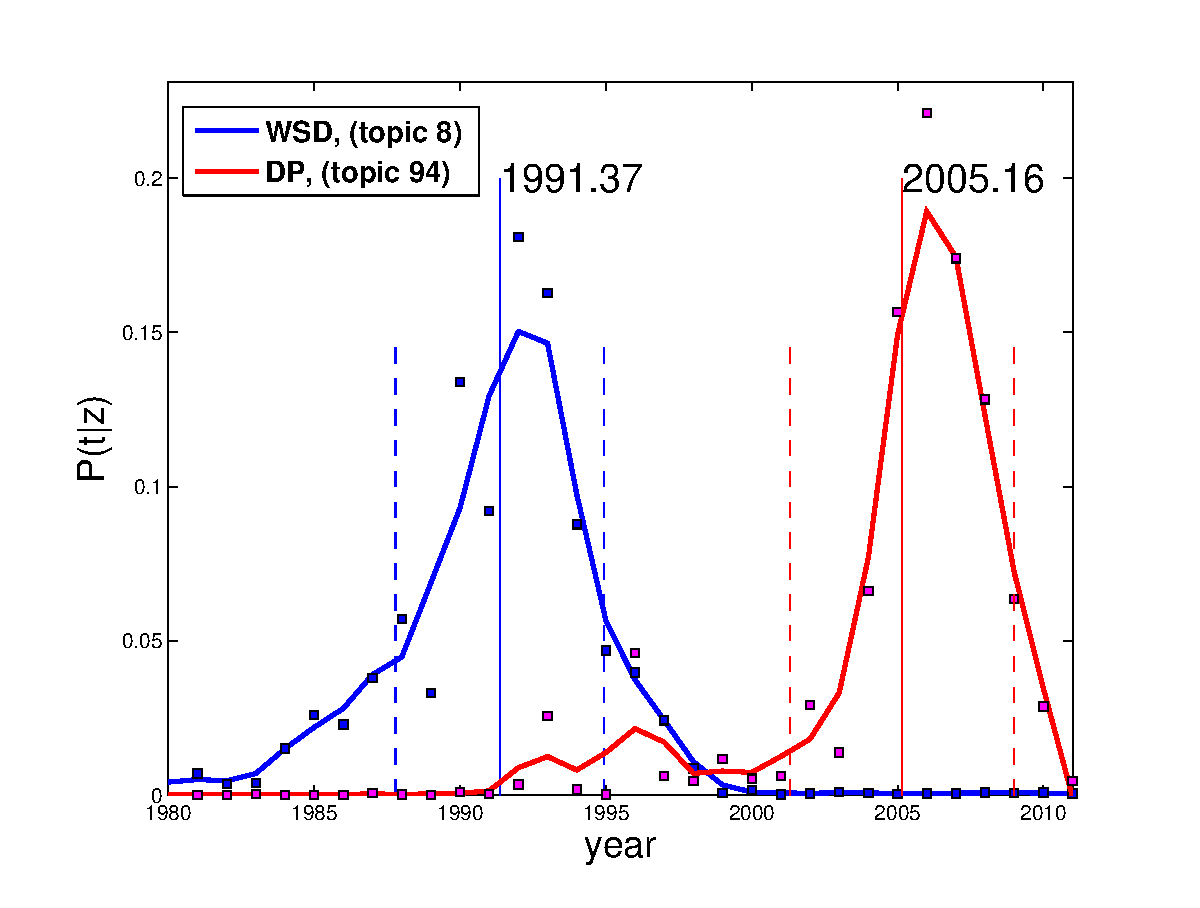
\includegraphics[scale= .5]{citation-lda/plot/aan_wsd_pd.eps}
  \end{center}
  \caption{Topic Temporal Strength for ``WSD'' and ``DP''}
  \label{fig::citation_aan_wsd_pd}
\end{figure}

\subsubsection{Discovering Temporal Strength}

To demonstrate that our model discovers the topic over time correctly, we show
the topic temporal strength of two topics, namely ``word sense
disambiguation''~(WSD) and ``dependency parsing''~(DP) from AAN in
\Cref{fig::citation_aan_wsd_pd}, and the computational details can be found in
\Cref{eq::citation_time1,eq::citation_time2,eq::citation_time3}.

In fact, the topic ``WSD'' was once a popular topic around early 90s while
``DP'' was newly popularized around year 2005. Based on our model, ``WSD'' has
the expected time $1991.37$, with a standard deviation $3.58$. For ``DP'', the
expectation is $2005.16$ and standard deviation is $3.84$. These estimations are
all consistent with the expert knowledge.

\subsubsection{Extracting Topic Keywords}

We list the extracted keywords~(phrases)~\footnote{Top word phrases are
generated from top 20 keywords and then matched with n-grams in titles of the
milestone papers} in \Cref{tab:aan,tab:pmc}. As will be explained in details
later, the topics are the dominant 10 topics in AAN and PMC datasets.  The
extracted keywords are mainly about the \emph{problem, task, model} and
\emph{methodology} of the topics.  For Topic~73 in AAN, it shows that the topic
investigates the problem of ``part-of-speech tagging'', models the problem as
``sequential labeling'', and approaches it with  ``discriminative parsing''
methods.  For Topic~61 in PMC, the nature of the topic can be recovered as
research on the risks of ``children exposure'' against ``agricultural spraying''
such as ``pesticides'' and ``organophosphorus''. In general, it is easy to
conclude the research problems or detailed methodology for each topic through
the extracted keywords along.  Besides, based on the spotted keywords, Topic~92,
Topic~96, Topic~80, and Topic~50 in AAN are all about the research theme
``statistical machine translation''.  But keywords reveal that topics differ
from each other as concerning about \emph{distinct} methods/models~(phrase-based
models~{\scriptsize (92)} \emph{v.s.} discriminative learning~{\scriptsize
(96)}) or problems~(reordering, alignment~{\scriptsize (80)} \emph{v.s.}
evaluation~{\scriptsize (50)}), which evidently substantiates that the keywords
are adequately discriminative even for quite related topics, serving as accurate
yet succinct summary for topics.

\begin{table*}
\caption{Dominant 10 Topics in AAN (100 topics)}\label{tab:aan}
\begin{center}
\begin{tabular}{|c|c|c|c|l|}
\hline %timesorted topic
Topic 	& Weight	 	&$\mathbf{E}(t)$ & $\mathrm{stdev}(t)$ &
  Top Keyword Phrases\\ \hline \hline
94		& 0.02806	& 2005.16		& 3.84	&
  dependency parsing, non-projective, shared tasks, multilingual\\
89		& 0.02761	& 2004.64		& 3.25	&
  sentiment classification, opinion analysis, orientation, learning \\
8		  & 0.02509	& 1991.37	  & 3.58	&
  word sense disambiguation, lexical semantics \\
92		& 0.02428	& 2004.98		& 3.26	&
  machine translation, phrase-based models, alignment \\
96		& 0.02277	& 2005.45		& 3.59	&
  machine translation, online, margin, discriminative learning \\
84		& 0.02093 & 2003.94		& 3.36	&
  semantic role labeling, shared tasks \\
80		& 0.02069	& 2003.44		& 3.83	&
  machine translation, reordering, alignment \\
73		& 0.01965	& 2002.76		& 4.09	&
  discriminative parsing, sequential labeling, part-of-speech \\
50		& 0.01908	& 2000.87		& 4.13	&
  machine translation, minimum error rate training, BLEU evaluation \\
72		& 0.01804	& 2002.74		& 4.45	&
  coreference resolution, machine learning, anaphora, pronoun \\ \hline\hline
\end{tabular}

\caption{Dominant 10 Topics in PMC (500 topics)}\label{tab:pmc}
\begin{tabular}{|c|c|c|c|l|}
\hline
Topic 	& Weight	&$\mathbf{E}(t)$ & $\mathrm{stdev}(t)$ &
  Top Keyword Phrases\\ \hline \hline
484		& 0.00624	& 2006.45	&8.95		&
  protein, molecular interaction, biomolecular, database\\
499		& 0.00504	& 2007.36	&9.89		&
  ensemble, gene, genome, resources \\
488		& 0.00478	& 2006.48	&19.37	&
  gnome-scale metabolic reconstruction, escherichia coli, malaria\\
175		& 0.00450	& 2004.48	&10.67	&
  air pollution, ambient particulates, heart rates, exposure\\
373		& 0.00388	& 2005.35	&11.77	&
  non-coding RNA, sequence alignment, structure prediction, genome \\
492		& 0.00382	& 2006.56	&11.39	&
  sorcerer II, global ocean sampling, metagenomics, atlantic \\
61		& 0.00351	& 2003.22	&12.12	&
  children exposure, agricultural spraying, pesticides, organophosphorus \\
2		& 0.00350	& 1998.00	&13.85		&
  yeast, actin,saccharomyces cerevisiae, protein, myosin, cell \\
38		& 0.00338	& 2002.67	&12.78		&
  cell,	regulatory T cell, CD4, CD25, human, Foxp3, expression, induction \\
86		& 0.00320	& 2003.64	&14.12		&
  phthalate exposure, human, urine, infants, metabolites, prenatal, health \\
  \hline\hline
\end{tabular}
\end{center}
\end{table*}

\subsection{Results of Theme Evolution Discovery}

\subsubsection{Identifying Important Topics}

As earlier implied, \Cref{tab:aan,tab:pmc} show the dominant 10 topics for AAN
and PMC, which are selected based on the topic weight $\{\hat\Pr(z=k)\}$ as
computed in \Cref{eq::citation_eq_topwei}. Identified dominant topics cover
major research progress and interest in NLP and life sciences. In AAN,  it is
obvious that the research theme ``statistical machine translation'' plays the
most important role in the community, thriving and diverse with multiple
different topics such as Topic~92, 96, 80, and 50. In PMC, many topics related
to ``public health'' are dominant such as Topic~175, 61, and 86, though the
detailed research topics are distinguishable from the keywords.

\begin{figure}[h!]
  \centering
  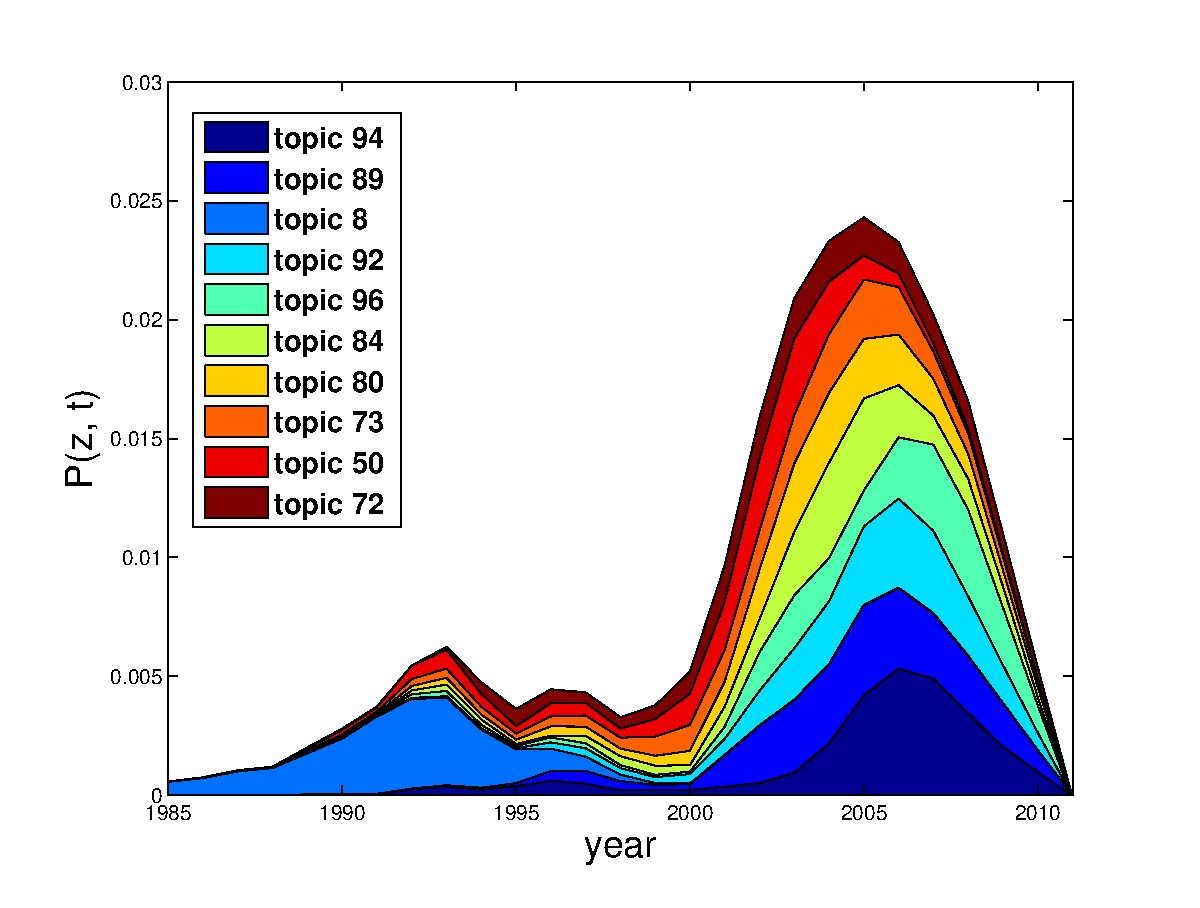
\includegraphics[scale=0.60
    ]{citation-lda/plot/AAN_10_temporal_stack_joint_smooth.eps}
  \caption{Topic-Temporal Joint Strength In AAN}\label{fig:tt_aan}
  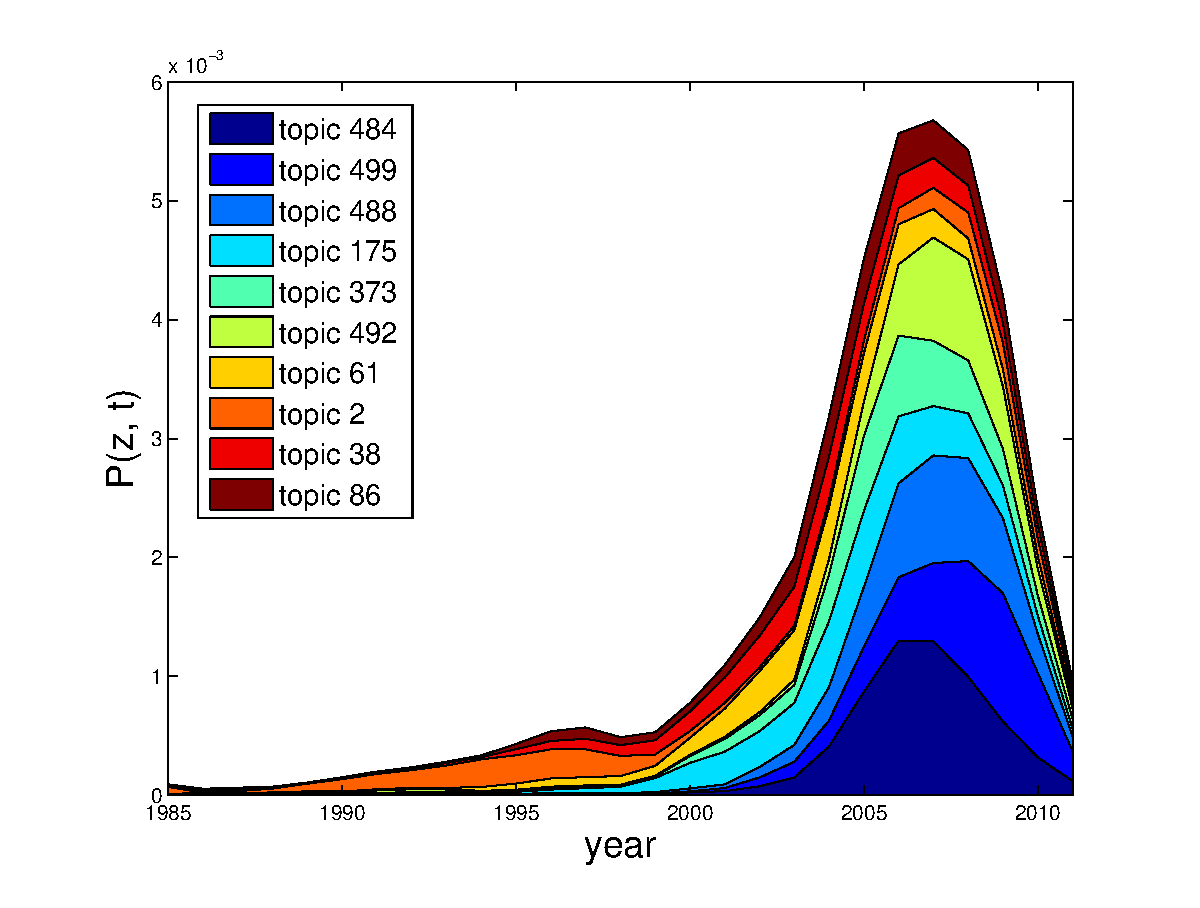
\includegraphics[scale=0.60
    ]{citation-lda/plot/PMC_10_temporal_stack_joint_smooth.eps}
  \caption{Topic-Temporal Joint Strength In PMC}\label{fig:tt_pmc}
\end{figure}

Taking the topic temporal strength into account,  $$\Pr(z=k,time=t) = \Pr(time =
k | z = k) \cdot \hat\Pr(z = k)$$ is the joint probability of topic strength and
time, allowing us to compare the topic strength in different time periods
\emph{with each other topics}. We visualize this for AAN and PMC in
\Cref{fig:tt_aan,fig:tt_pmc}, and it shows that the major research development
occurred after year 2000 for both two dataset~\footnote{However, there is
  possibility that our datasets are biased as being rich in citations after year
2000}, except that Topic 8 (``word sense disambiguation'') of AAN was dominant
compared with others in early 90s while Topic 2 of ``yeast'', ``saccharomyces
cerevisiae'' in PMC was a extensively studied around entire 90s.

\subsubsection{Topic Dependency \& Evolution Patterns}

\begin{figure}[h!]
  \begin{center}
  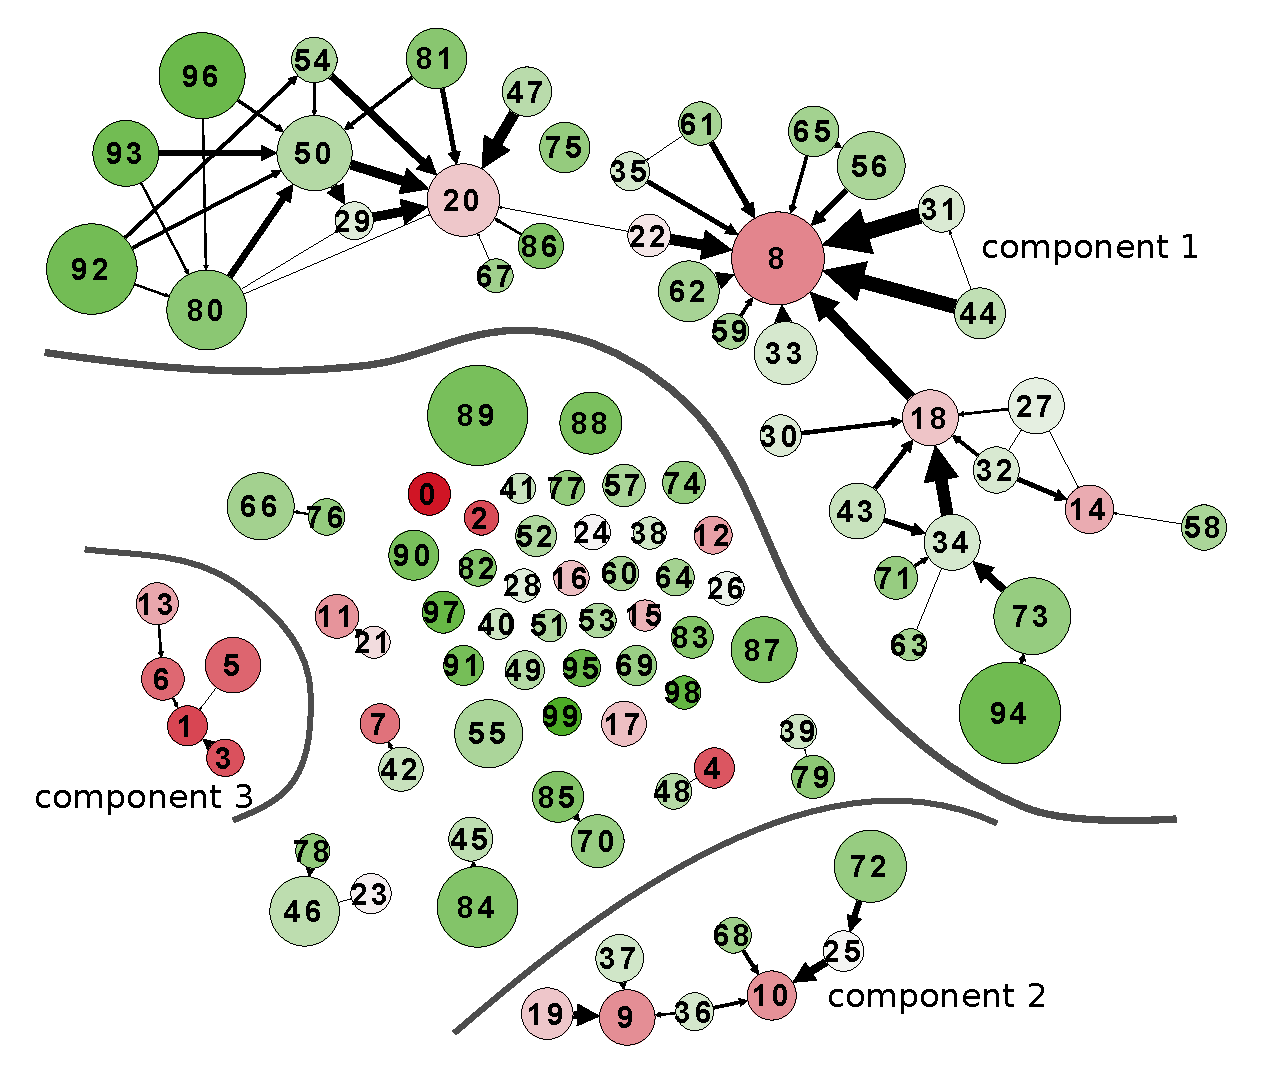
\includegraphics[scale=.7]{citation-lda/plot/full_color_with_labels}
  \caption{Theme Evolution Graph of AAN}
  \label{fig:full}
  \end{center}
\end{figure}

After applying the pruning to the \emph{topic level citation structure} the
evolution graph for research themes can be plotted.  We show the evolution graph
of AAN with 100 topics in \Cref{fig:full}: each node represents a topic
and the importance of topics are discriminated by the size of nodes. The green
nodes are new topics while the red ones are \emph{relatively} old. In addition,
the dependency between topics are reflected by the thickness of edges .

There are three major connected component, each of which contains themes
developing over time: Component 3 is about the theme ``grammar'', and
corresponding topics entirely \emph{faded out} during early 90s. Nevertheless,
Component 2 has the theme of ``discourse/dialogue'' and ``summarization'',
showing mildly progress recently (e.g., Topic 72~(2003) of \emph{``machine
learning'' based ``coreference resolution''}).  Observing the Component 1, which
is the largest, is interesting with discovery of various theme evolution
patterns: Topic 8~(1991) about ``word sense disambiguation'' was \emph{branched}
into many topics, with one of them (Topic 18) being about ``prepositional phrase
attachment''~(1994).  Soon, Topic 18 further enabled Topic 34~(1999) of
``statistical parsing'', and again Topic 73 of ``discriminative parsing'' was
established by 2003 on top of Topic 34. Later, Topic 94 of ``dependency
parsing'' raised and has grown as one dominant topic since 2005.

\begin{table*}[t!]
\caption{SMT Example for Theme Evolution}
\label{tab:smt_ex}
\begin{center}
\begin{tabular}{|c|c|c|l|l|}
\hline
Topic &Year & Paper ID & Paper Title & $\hat\varphi$ \\ \hline \hline
\multirow{4}{*}{Topic 20}
%Cluster 17 Time 20
          & 1990 & P1 &
  A Statistical Approach To Machine Translation & $0.036542$ \\
					& 1991 & P2 &
  A Program For Aligning Sentences In Bilingual Corpora & $0.047619$ \\
					& 1993 & P3 &
  The Mathematics Of Statistical Machine Translation: &\\
  &&& \; Parameter Estimation & $0.060931$\\
  \hline
%Cluster 28 Time 29
\multirow{3}{*}{Topic 29} 	& 1996 & P4 &
  HMM-Based Word Alignment In Statistical Translation & $0.097162$\\
					& 1997 & P5 &
  Decoding Algorithm In Statistical Machine Translation & $0.030390$\\
					& 1999 & P6 &
  Improved alignment models for statistical machine translation & $0.036367$\\
  \hline
%Cluster 56 Time 50
\multirow{7}{*}{Topic 50}
          & 2002 & P7 &
  BLEU: A Method For Automatic Evaluation Of Machine &\\
  &&& \; Translation & $0.087902$ \\
          & 2002 	& P8 	&
  Discriminative Training \& Maximum Entropy Models For &\\
  &&& \; Statistical Machine Translation & $0.027799$\\
					& 2003 & P9 &
  Minimum Error Rate Training In Statistical Machine & \\
  &&& \; Translation & $0.027027$\\
  \hline
%Cluster 39 Time 93
\multirow{4}{*}{Topic 93}
          & 2003 & P10&
  Statistical Phrase-Based Translation & $0.036239$\\
					& 2005 & P11&
  A Hierarchical Phrase-Based Model For Statistical Machine &\\
  &&& \; Translation & $0.022442$ \\
					& 2007 & P12&
  Hierarchical Phrase-Based Translation & $0.043163$\\
  \hline\hline
\end{tabular}
\end{center}
\end{table*}

Another key thread of theme in Component 1 was initiated by Topic 20, which was
the very beginning topic of the theme ``statistical machine translation''~(SMT).
The topics along the theme evolution path are presented in \Cref{tab:smt_ex},
including 4 topics~(Topic 20, 29, 50, and 93), together with the milestone
papers~(top 3 for each). In addition, the temporal distribution over time is
given in \Cref{fig:smt_temporal}, where the citations among the milestone
papers, and the dependency strength between consecutive topics are also
depicted.


\begin{figure}[h!]
  \begin{center}
    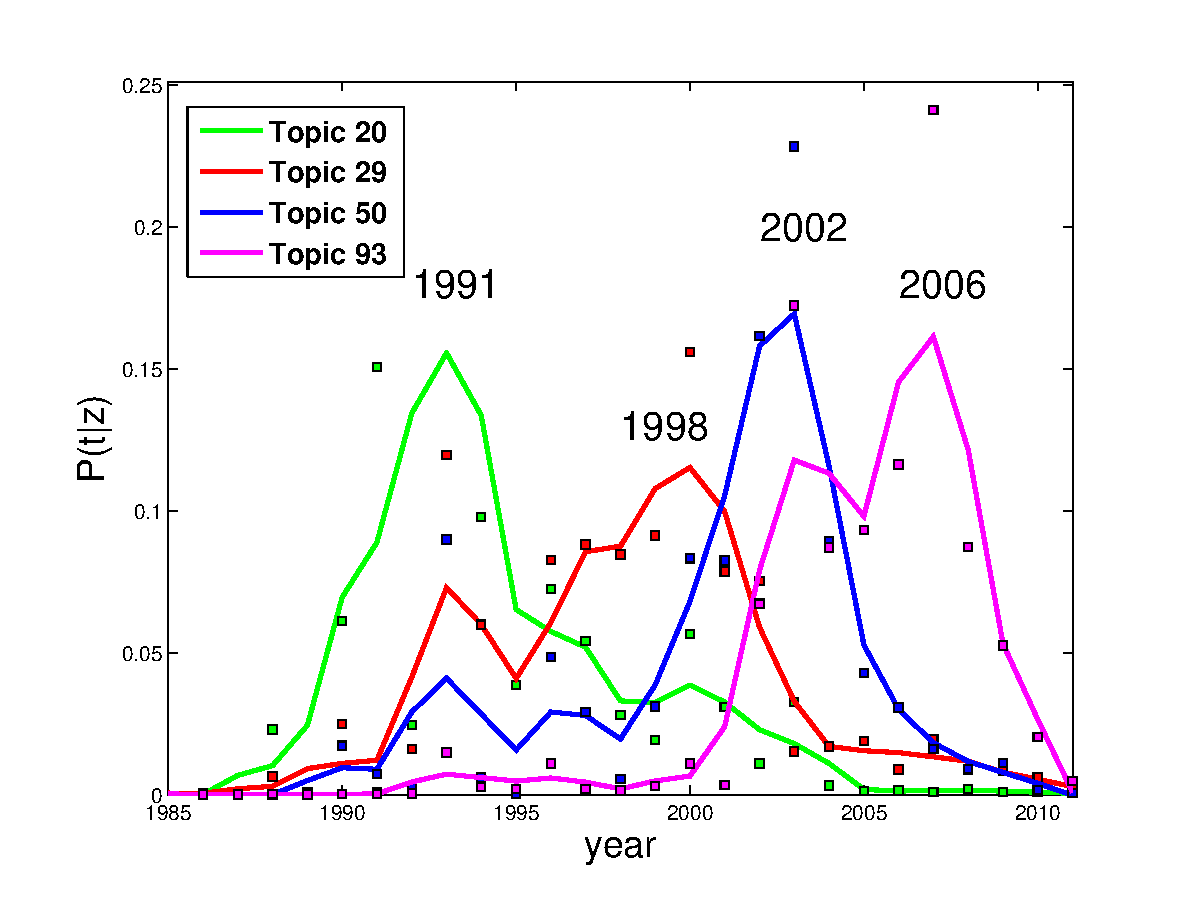
\includegraphics[scale= .6]{citation-lda/plot/smt_4topic_temporal}
    ~
    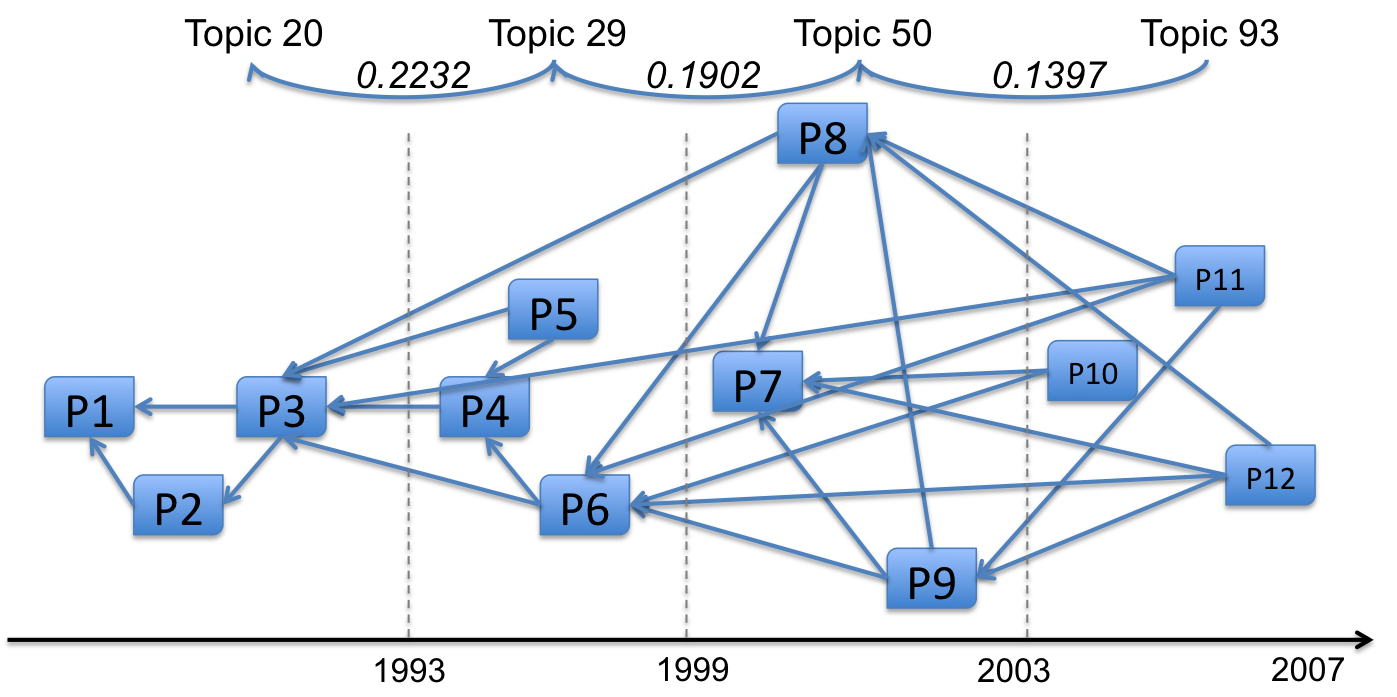
\includegraphics[scale= .45]{citation-lda/plot/smt_milestone_link}
  \end{center}
  \caption{Temporal Evolution in Topics of Theme SMT}\label{fig:smt_temporal}
\end{figure}

Specifically, Topic~20 began increasing its impact around early 90s, introducing
basic statistical methods to machine translation; Later, around 1998, its
popularity was shifted to Topic~29 which was specialized in subproblems such as
``decoding'', ``alignment'' and ``reordering'' in SMT; By 2002, however, Topic
50 emerged, and soon grew as the new dominant topic by proposing ``BLEU'' as the
standard evaluation metric and investigating ``discriminative methods'' such as
``minimum error rate training''; The current state of the art approach in SMT,
``phrase-based model'', accompanied by the raise of Topic~93, was actually built
on top of previous work, especially milestone papers of $P7$-$P9$ of Topic~50.

In \Cref{fig:smt_temporal}, citation links among milestone papers across topics
are illustrated, which clearly show the formation of topics through the ``stable
core set'' of milestone papers that \emph{get cited together}~(co-cited). More
importantly, it is evident that the ``co-citation'' of ``core'' papers is the
direct contributing factor in the dependency relation between two consecutive
topics.

\subsection{Model Selection \& Comparison Results}
\label{sec::citation_sec_model_selection}

We now discuss how to select the topic numbers for Citation-LDA and compare the
performance with Content-LDA on two metrics, namely, \emph{Forward Citation} and
\emph{Jounral Conditional Entropy}.

We investigate the conventional Content-LDA~\cite{blei2003latent} as our
baseline, using the title and abstract to represent the papers in both datasets.
In order to make the output of Content-LDA aligned with that of Citation-LDA, we
need to derive the missing \emph{topic-doc} distribution: the distribution over
papers (instead of tokens) for each topic.  As in our experiments, we assume
{$\Pr(d | k) \propto \Pr(k | d) \cdot \Pr(d)$} whereas {$\Pr(d)\propto |d|$}
with {\scriptsize $|d|$} being the document length for $d$.

\subsubsection{Evluation on Forward Citation for AAN}

We compute the \emph{topic forward citation} probability based on the topic
dependency~(\Cref{eq::citation_lda_citation_structure}) and expected topic
time~(\Cref{eq::citation_time3}).  In words, the forward citation probability
reflects the chance a topic \emph{cites} future topics that arise after
itself~(though it is impossible for a paper to cite a future paper).  We compute
the model's loss on topic $k$ by the topic \emph{future citation probability} ,
which is given by: {$l(k) = \sum\limits_{\tilde{k}, t(\tilde{k}) > t(k)} \Pr(k
\rightarrow \tilde{k} | k)$} for topic $k$. To assess the total \emph{loss for
Forward Citation} of a model, we define it as follows:

 $$\mathrm{Loss}_{FC} = \sum\limits_k \Pr(k) \cdot l(k)$$

\begin{table}[h!]
\caption{Loss on Forward Citation~(AAN)}
\label{tab::citation-fc}
\begin{center}
\begin{tabular}{|c|c|c|c|}
\hline
\#topic	&	20	&	100	&	200 \\
\hline\hline
Citation-LDA 	& 0.3148		&	\textbf{0.1917}	&	0.2488	\\
Content-LDA		& 0.3745		&	0.3816	&	0.3924	\\
\hline \hline
\end{tabular}
\end{center}
\end{table}

We show the evaluation based on \emph{Forward Citation} for AAN in
\Cref{tab::citation-fc}, from which we see: 1) Citation-LDA has better
performance on Forward Citation compared with Content-LDA and 2) 100 topics are
a good choice for AAN dataset.

\subsubsection{Evaluation on Journal Conditional Entropy for PMC}

As discussed before, the journal sources are fairly good ``coarse'' annotation
for topics in PMC. For topic $k$, we can derive the \emph{journal conditional
  distribution on topic $k$}, yielding the conditional entropy~\footnote{Entropy
$H(X) = - \sum\limits_{x} \Pr(x) \log \Pr(x)$}:  $$H(J | z) =
\sum\limits_{z=k} \Pr(z=k) \cdot H(J | z=k)$$ The $H(J | z)$ would have low
value if the journal labels and topic labels are \emph{consistent}, by which
we mean that for papers with the \emph{same topic label}~(in a probabilistic
sense), there is \emph{one journal label} being as dominant as possible,
ideally being purely the only journal label. Hence, we can compute the
\emph{loss for Journal Conditional Entropy} of a model as:

$$\mathrm{Loss}_{CE} = H(J|z)$$

\begin{table}[h!]
\caption{Loss on Journal Conditional Entropy~(PMC)}
\label{tab::citation-ce}
\begin{center}
\begin{tabular}{|c|c|c|c|c|}
\hline
\#topic	&	100	& 300 &	500	&	1000 \\
\hline\hline
Citation-LDA 	& 	3.5047	&	3.2144	&	\textbf{3.18729}	&	3.4118\\
Content-LDA		& 	4.2048	& 	4.2805	&	4.06496	&	4.4725\\
\hline \hline
\end{tabular}
\end{center}
\end{table}

Based on the journal conditional entropy on
topics~(\Cref{tab::citation-ce}), we again demonstrate the advantage of
Citation-LDA over Content-LDA: the topic formed in Citation-LDA is more
consistent with the ``journal labels'' than Content-LDA. In addition, we verify
that for PMC dataset, 500 topics might be a reasonable choice.


\section{Notes and Conclusion}\label{sec::citation-conclusion}

In this chapter, we proposed a novel approach for analyzing research theme
evolution of scientific literature data where citation links are available.  1)
to discover research topics, which includes finding milestone papers, computing
topic temporal strength, and extracting keywords for topics; 2) to discover
theme evolution, which includes identifying topic importance, learning topic
dependency relation, and recognizing the evolution patterns.  These
computational components together enable us to understand evolution of research
themes by constructing the evolution graph.  In experiments, we investigated two
datasets, namely AAN and PMC from two domains, with extensive results showing
that our proposed model, Citation-LDA, which represents article paper as ``bag
of citations'' and model the generation of citation links within a probabilistic
framework, can effectively accomplish the tasks defined above, with the
performance better than Content-LDA.  Our proposed Citation-LDA, together with
the developed mining techniques, can be very useful to help researchers digest
literature quickly, thus speeding up scientific research discovery and
delivering very broad positive impact on the society.

In general, our model can also be applied to any graph data for tasks such as
network clustering and ranking, as well as modeling the evolution of network
generation, which we leave as future work directions.
